% 圆周运动的速度

\subsection{几何法}
\pentry{小角正弦值极限\upref{LimArc},速度的定义\upref{VnA}}

\begin{figure}[ht]
\centering
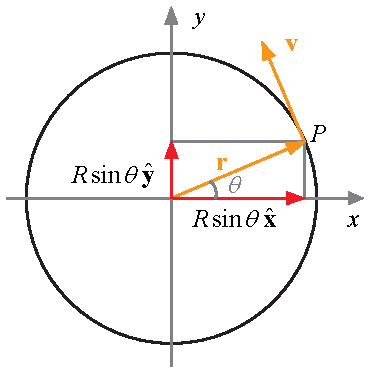
\includegraphics[width=6.3cm]{./figures/CMVD1.pdf}
\caption{匀速圆周运动的速度} \label{CMVD_fig1}
\end{figure}

如图设一个点 $P$ 做半径为 $R$ 的圆周运动, 角速度为 $\omega $(可以是时间的函数), 那么在一段微小时间 $\Delta t$ 内, 可以认为 $\omega$ 是常量, 点 $P$ 转过的角度为 $\Delta \theta  = \omega \Delta t$. 这样,根据小角正弦值极限\upref{LimArc},当 $\Delta t \to 0$ 时, 点 $P$ 在 $\Delta t$ 内走过的位移长度(线段的长度)趋近于弧的长度,即 $\abs{\Delta \bvec s} \to R\omega \Delta t$.  

根据速度的定义
\begin{equation}
\bvec v = \lim_{\Delta t \to 0} \frac{\Delta \bvec s}{\Delta t}
\end{equation}
速度的大小为
\begin{equation}
v = \lim_{\Delta t \to 0} \frac{\abs{\Delta \bvec s}}{\Delta t} = \lim_{\Delta t \to 0} \frac{\omega R \Delta t}{\Delta t} = \omega R 
\end{equation}
速度的方向显然与过 $A$ 点的圆的切线重合.

\subsection{求导法}
\pentry{矢量的导数\ 求导法则\upref{DerV}}
如图,在平面直角坐标系(单位矢量分别为 $\uvec x$,  $\uvec y$ )中,令一个绕原点做逆时针匀速圆周运动的质点的位矢为 $\bvec r$, 与 $\uvec x$ 的夹角是时间的函数 $\theta(t)$, 圆周运动的半径为 $R$. 那么任意时刻 $t$ 将位矢 $\bvec r$ 沿着 $x$ 与 $y$ 轴方向分解,有
\begin{equation}\label{CMVD_eq1}
\bvec r(t) = R\cos \theta(t)\, \uvec x + R\sin\theta(t)\, \uvec y
\end{equation}
其中 $\uvec x$ 是 $x$ 轴正方向的单位矢量, $\uvec y$ 是 $y$ 轴正方向的单位矢量. 由速度的定义 $\bvec v = \dv*{\bvec r}{t}$, 即
\begin{equation}\label{CMVD_eq2}
\ali{
\bvec v &= \dv{t} ( R\cos \theta\, \uvec x + R\sin\theta \, \uvec y)
= - R\dot\theta \sin\theta\, \uvec x + R\dot\theta \cos \theta\, \uvec y\\
&= \dot\theta R [\cos(\theta + \pi/2) \uvec x + \sin(\theta + \pi/2)\uvec y]
}\end{equation}
定义\textbf{瞬时角速度}(简称\textbf{角速度})等于 $\theta$ 关于时间的导数 $\omega = \dot \theta$, 则速度大小为 $v = \omega R$, 方向为 $\uvec r$ 逆时针旋转 $\pi/2$, 即圆的切线方向.

\subsection{三维空间的情况}
\pentry{矢量叉乘\upref{Cross}}

\begin{figure}[ht]
\centering
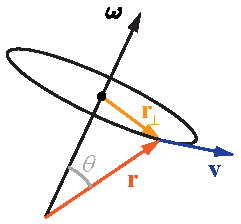
\includegraphics[width=4.2cm]{./figures/CMVD2.pdf}
\caption{角速度与线速度} \label{CMVD_fig2}
\end{figure}

如\autoref{CMVD_fig2}, 在三维空间中, 圆周运动所在的平面可以任意选取, 我们可以将角速度拓展成一个矢量 $\bvec\omega$, 其方向垂直于该平面并由右手定则\upref{RHRul} 确定. 令坐标系的原点在圆周运动的轴上, 用位矢 $\bvec r$ 表示点 $P$ 的位置, 则圆周运动的半径为 $r_\bot = r \sin\theta$, 其中 $\theta$ 是 $\bvec r$ 与 $\bvec \omega$ 的夹角. 所以圆周运动速度的大小为 $v = \omega r \sin\theta$. 根据矢量叉乘的几何定义\upref{Cross}, 有
\begin{equation}\label{CMVD_eq5}
\bvec v = \bvec\omega \cross \bvec r
\end{equation}
